% Informe autocontenido; compilar mediante main.tex.
\section{Problema y alcance}
Este trabajo construye un entorno que genera problemas cuantitativos en español
y comprueba automáticamente las respuestas de modelos de lenguaje. El objetivo
es preparar datos y una función de recompensa para entrenar posteriormente a
Qwen3-1.7B, sin realizar entrenamiento en esta entrega. Cada problema proporciona
fórmulas y equivalencias de unidades para evaluar cálculo y composición de
operaciones, en lugar de memoria de conocimientos físicos.

El estudio utiliza 180 tareas repartidas entre entrenamiento, validación y
prueba. Primero se define cómo generarlas y verificarlas, luego se calibra su
dificultad con el modelo objetivo y finalmente se producen datos de entrenamiento
y se mide el desempeño inicial. Se comparan Qwen3-1.7B, Llama 3.2-1B y
SmolLM2-1.7B-Instruct con Qwen3-8B, que también genera soluciones como modelo
profesor, y con DeepSeek-V4-Pro-0813 como referencia externa. Todos responden
en un turno, sin calculadora, intérprete ni otras herramientas.

\section{Diseño del dataset}
Llamamos \emph{familia} a un tipo de problema definido por sus magnitudes y
fórmula. Las tres familias son una elección de este trabajo, no categorías
impuestas por el desafío: velocidad, $v=d/t$; energía cinética, $E=mv^2/2$;
y luminosidad, $L=4\pi d^2F$. Aquí $d$ es distancia, $t$ tiempo, $m$ masa,
$v$ velocidad, $E$ energía, $L$ luminosidad y $F$ flujo de energía recibido por unidad de superficie.
Permiten contrastar una división con cálculos que incorporan cuadrados y
productos, manteniendo respuestas verificables por código.

Cada familia combina dos estructuras: datos directos o suma de dos componentes
positivos, como $d_1+d_2$, $m_1+m_2$ o $F_1+F_2$. Sobre cada problema físico
se construyen tres tareas equivalentes: fácil usa unidades del Sistema
Internacional (SI) sin conversiones, media convierte una entrada y difícil
convierte dos entradas y, en velocidad y energía, también la salida. En
luminosidad difícil se mantiene la salida en W, por lo que hay dos conversiones.
Estos niveles describen operaciones previstas, no garantizan un orden de
dificultad para todos los modelos.

El generador, incluido en \path{code/src/challenge/generator.py} del paquete,
muestrea distancias de 101--9999 m y tiempos de 7--199 s para velocidad, masas
de 1,1--49,9 kg y velocidades de 1,1--49,9 m/s para energía, y distancias
enteras de 2--30 m con flujos de 0,01--0,99 W/m$^2$ para luminosidad. Las
sumas reparten el total en fracciones entre 0,2 y 0,8, y los valores se imprimen
con hasta 15 cifras significativas. Se excluyen cero, negativos e incertidumbres
físicas. La generación reproducible y la sensibilidad a variantes tienen como
antecedentes Reasoning Gym, de Stojanovski et al. (2025)~\cite{reasoninggym}, y
GSM-Symbolic, de Mirzadeh et al. (2024)~\cite{gsmsymbolic}.

Se generan 20 problemas físicos por familia con semilla 4301 y se distribuyen
con semilla 4302, manteniendo juntas sus tres variantes para evitar que una
misma situación aparezca tanto en entrenamiento como en prueba. Así se obtienen
60 problemas físicos y $60\times3=180$ tareas. La tabla~\ref{tab:dataset}
explicita el reparto, elegido antes de evaluar para cubrir cada combinación de
familia y nivel con una carga de inferencia local acotada.

\begin{table}[ht]
\centering
\begin{tabular}{lrrrr}
Partición & Problemas por familia & Tareas por familia & Por nivel/familia & Total \\
\midrule
Train & 10 & 30 & 10 & 90 \\
Eval & 4 & 12 & 4 & 36 \\
Test & 6 & 18 & 6 & 54 \\
\midrule
Total & 20 & 60 & 20 & 180 \\
\end{tabular}
\caption{Cada partición contiene las tres familias y conserva juntas las variantes
fácil, media y difícil de cada problema. Las estructuras directa y suma se balancean.}
\label{tab:dataset}
\end{table}

Train se usa para generar soluciones y pares de preferencias para entrenamiento,
eval queda reservado para validación y test mide el desempeño final. Ningún problema utilizado durante
el desarrollo o la calibración integra estas particiones. Las plantillas sí
son compartidas, por lo que se evalúan nuevas magnitudes y combinaciones,
no generalización a otros tipos de problemas o redacciones arbitrarias.

Como muestra de una tarea de velocidad de nivel medio, se entregan $d_1=4{,}08$ km,
$d_2=1{,}02$ km, $t=88$ s y la fórmula $v=(d_1+d_2)/t$, y se pide el resultado
en m/s. Tras convertir las distancias, la respuesta esperada es $5100/88$
m/s y una salida válida es \verb|{"value":57.95,"unit":"m/s"}|.
Cada tarea solicita hasta 80 palabras de explicación y un único resultado final.
Para decidir automáticamente si esa salida es correcta se aplica el siguiente
procedimiento, común a todos los modelos.

\section{Verificación de respuestas y limitaciones}
La función \texttt{reward(prompt, completion)} recibe el enunciado y la respuesta
del modelo y devuelve 1 si la considera correcta o 0 en caso contrario. Los
resultados esperados se calculan mediante las fórmulas del generador y se
comprueban con un segundo cálculo que interpreta los datos impresos en el
enunciado, usando tolerancia relativa $10^{-10}$. Se guardan por separado en
\path{data/tasks/private/}: son referencias de evaluación que el modelo no
recibe. Antes de llamar a \texttt{reward}, el programa
consumidor lee esos archivos y registra las tareas con \texttt{load\_tasks},
función incluida en \path{code/src/challenge/verifier.py}. Un enunciado no
registrado produce \texttt{ValueError}, que indica un error de integración.

El extractor identifica un resultado final en JSON con número y unidad o como
cantidad seguida de unidad, sin consultar la solución ni ejecutar expresiones.
Después convierte la cantidad a SI, por ejemplo de km/h a m/s, y comprueba
que corresponda a la magnitud pedida y sea finita. Si $y$ es el valor obtenido
y $y^*$ el esperado, ambos en SI, la condición de aceptación es
$|y-y^*|\leq0{,}01|y^*|$. Esta tolerancia del 1\% admite redondeo, pero no
certifica la explicación. Se admiten m/s y km/h para velocidad, J, kJ y erg
para energía, y W, kW, erg/s y luminosidades solares para luminosidad.

Las respuestas se clasifican como correctas (\texttt{correct}), numéricamente
incorrectas (\texttt{numeric}), de magnitud incompatible (\texttt{unit}) o no
interpretadas (\texttt{unparsed}). Esta última categoría aparece ante formatos
no reconocidos, resultados ambiguos o ausencia de una cantidad final admisible,
y no demuestra un error matemático. La \emph{cobertura} es la proporción de
respuestas que el extractor logra interpretar. También se registran las salidas
cortadas por el límite de generación y los intentos incompletos, sin excluirlos
del cálculo de resultados.

El código de verificación entregado se fijó antes de iniciar test y no se
modificó al observar sus respuestas. Las pruebas incluyen
cantidades equivalentes como 22 m/s y 79,2 km/h y rechazos de alternativas,
resultados contradictorios, unidades incompatibles, claves JSON duplicadas y
números no finitos, sin rescatar un valor previo por coincidir con la solución.

Persisten tres límites importantes. Primero, se acepta una unidad físicamente
equivalente aunque difiera de la solicitada, lo que permite omitir la conversión
de salida. Exigirla reduciría los aciertos de Llama de cuatro a tres. Segundo,
coma y punto se leen como decimales, de modo que \texttt{1,000 J} significa 1 J,
sin que el enunciado descarte explícitamente separadores de miles. Además, alias
como \texttt{joule}, \texttt{kph} y \texttt{Km/h}, números en palabras, ciertos
superíndices y expresiones LaTeX quedan sin interpretar. Tercero, aunque la
inferencia limita la salida a 1024 tokens, la función de recompensa no impone
su propio máximo de longitud.

También se confirmaron siete falsos negativos entre el objetivo y el profesor
por líneas intermedias que invalidan un JSON final numéricamente correcto.
Este diagnóstico posterior a test no cambia las métricas ni valida el razonamiento. Para mostrar cuánto podría afectar la extracción, las tablas
incluyen una cota optimista que supone correctas todas las respuestas no
interpretadas, sin presentarla como intervalo de confianza. Antes de entrenar
será necesario ampliar las pruebas y precisar las reglas de formato y unidad,
y cualquier evaluador ajustado con estos casos deberá medirse sobre un nuevo
conjunto reservado si se desea una evaluación independiente.

\section{Calibración y protocolo experimental}
Una vez definido el verificador, se comprobó si las tareas daban al objetivo
Qwen3-1.7B una mezcla de aciertos y errores que justificara entrenarlo después.
Para ello se realizaron pruebas preliminares separadas del dataset final y se
ajustó luminosidad, cuya proporción de aciertos estaba cerca de cero. Se
redujeron sus magnitudes y se eliminó la conversión de salida del nivel difícil,
repitiendo la generación de respuestas cuando cambiaba el enunciado.

El resultado consolidado de esta calibración reúne 30 problemas físicos,
10 por familia, con tres niveles cada uno: 90 tareas. Qwen3-1.7B respondió
tres veces cada tarea, produciendo $90\times3=270$ intentos. Se emplean tres
muestras para medir tanto el acierto de una respuesta individual (pass@1)
como la proporción de tareas resueltas al menos una vez entre tres intentos
(pass@3). Hubo 132 aciertos, 126 errores numéricos y 12 respuestas no
interpretadas, por lo que pass@1 fue $132/270=48{,}89\%$, pass@3 fue
$59/90=65{,}56\%$ y la cobertura fue $258/270=95{,}56\%$. Los tres
truncamientos observados permanecieron en esos denominadores.

\begin{figure}[ht]
\centering
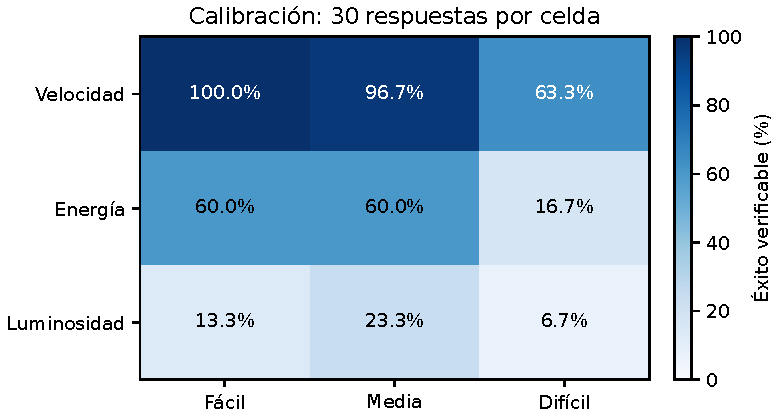
\includegraphics[width=.85\linewidth]{final-v2/figures/calibration.pdf}
\caption{Calibración de Qwen3-1.7B antes de fijar el test. Cada combinación de
familia y nivel contiene 10 tareas y 30 respuestas.}
\end{figure}

Luminosidad difícil conservó solo 2/30 aciertos y se mantuvo para estudiar una
condición especialmente exigente, mientras velocidad fácil alcanzó 30/30 y
sirvió como control sencillo. Velocidad difícil obtuvo 19/30, y los promedios
fácil y medio fueron 57,78\% y 60,00\%. Hay señal de acierto y error global,
pero no calibración suficiente en todas las combinaciones ni un orden estricto
entre niveles. Con estas limitaciones se fijaron las tareas finales y el
procedimiento empleado tanto para generar datos como para medir la línea base.

Las inferencias locales se ejecutaron de forma secuencial en un equipo Intel
Core 5 210H con 12 CPU lógicas, 30,47 GiB de RAM y GPU RTX 3050 Laptop de
6 GiB, usando Ollama 0.18.0 y Python 3.12.13. Se utilizaron pesos en formato
GGUF con cuantización Q4\_K\_M para ambos Qwen y SmolLM2, y Q8\_0 para
Llama, formatos que reducen la memoria necesaria con distinta precisión
numérica. Las huellas de los pesos y sus licencias están en
\path{data/tasks/models.json}: Apache-2.0 para Qwen y SmolLM2 y Community
License para Llama~\cite{qwen17,qwen8,llama,smol}.

Para obtener respuestas variadas se usó temperatura 0,7 con top-p 0,9,
top-k 40 y min-p 0. El contexto fue de 2048 tokens y el máximo de salida
de 1024, con batch de 128, solicitud de 99 capas en GPU y
\texttt{think=false} para desactivar el modo de pensamiento. Cada petición
contenía un mensaje de usuario y no forzaba JSON. Las semillas 42, 43 y 44
controlaron el muestreo de las tres respuestas por tarea en la evaluación,
y 42--45 las cuatro del profesor para entrenamiento. Se conservaron respuestas,
tiempos y tokens para poder recalcular métricas sin nuevas inferencias,
aunque las semillas no garantizan igualdad entre motores o versiones.

\section{Datos derivados para entrenamiento posterior}
Con el diseño fijado, se usó exclusivamente train para crear dos productos:
soluciones verificadas para ajuste supervisado (SFT) y pares de respuesta
preferida y rechazada para optimización por preferencias (DPO). Las 90 tareas
de train se distribuyen en nueve combinaciones de familia y nivel, con 10
tareas por combinación. Qwen3-8B generó cuatro respuestas por tarea, es decir,
40 por combinación y $90\times4=360$ en total, una escala elegida para muestrear
variantes bajo el presupuesto de cómputo local.

El verificador aceptó 193 respuestas y clasificó las restantes como 154 errores
numéricos y 13 no interpretadas. Al eliminar repeticiones textuales por tarea,
ignorando diferencias de espacios, quedaron 178 candidatas para SFT. La revisión
comenzó con cinco por combinación, seleccionadas con semilla 4303, y se amplió
al detectar defectos hasta cubrir todas las candidatas. Se comprobó que datos,
conversiones y operaciones concordaran con el problema, reteniendo 121 y
descartando 57 por inconsistencias en el desarrollo. Esta revisión fue realizada
por agentes de IA y no constituye certificación humana. Las 121 soluciones
retenidas cubren 46 tareas y 20 problemas físicos.

Para DPO se emparejó una solución retenida con una respuesta inequívocamente
incorrecta del mismo enunciado, con hasta dos pares distintos por tarea para
limitar la repetición de ejemplos. Cuando el profesor no aportaba suficientes
respuestas incorrectas para ese emparejamiento, se consultó al objetivo. Esa
condición seleccionó 38 tareas de train y tres muestras por tarea produjeron
$38\times3=114$ respuestas adicionales: 89 correctas, 19 errores numéricos y
6 no interpretadas. Solo los errores explícitos podían actuar como respuestas
rechazadas, y al aplicar el límite de pares sin reutilizar sus miembros quedaron
35 pares de 25 tareas y 17 problemas físicos. De las 35 rechazadas, 22 proceden
del profesor y 13 del objetivo. Las cantidades finales son resultado del
filtrado y los emparejamientos disponibles, no cuotas rellenadas artificialmente.

\begin{table}[ht]
\centering
\begin{tabular}{llrr}
Familia & Dificultad & SFT & DPO \\
\midrule
Velocidad & Fácil & 27 & 3 \\
Velocidad & Media & 25 & 4 \\
Velocidad & Difícil & 22 & 11 \\
Energía & Fácil & 13 & 1 \\
Energía & Media & 10 & 5 \\
Energía & Difícil & 1 & 1 \\
Luminosidad & Fácil & 11 & 3 \\
Luminosidad & Media & 11 & 6 \\
Luminosidad & Difícil & 1 & 1 \\
\midrule
Total & & 121 & 35 \\
\end{tabular}
\caption{Soluciones SFT y pares DPO retenidos tras verificación y revisión.
Una tarea puede aportar más de una solución o par.}
\end{table}

El volumen queda por debajo de las metas orientativas de 4000 SFT y 2000 DPO
porque se priorizó revisar la calidad de una generación local acotada. Los 360
intentos del profesor tomaron 2537,21 s y 56563 tokens, con 7,05 s por respuesta.
A la tasa de retención observada, alcanzar 4000 SFT exigiría unas 23,30 horas
solo de inferencia del profesor. La escasez de una única solución en energía
y luminosidad difíciles limita el entrenamiento posterior, por lo que estos
datos preparan el experimento pero no demuestran suficiencia para aprender.
La siguiente evaluación mide el desempeño previo a cualquier entrenamiento.

\section{Línea base y análisis cualitativo}
El conjunto test reúne seis problemas físicos por cada una de las tres familias,
es decir, 18 problemas. Cada uno tiene tres niveles, de donde surgen las
54 tareas. Se obtuvieron tres respuestas por tarea y modelo, equivalentes a
162 intentos por modelo y 648 entre los cuatro locales. Pass@1 estima qué
proporción de respuestas individuales es correcta, mientras pass@3 indica en
qué proporción de tareas al menos uno de los tres intentos acierta, mostrando
el beneficio de disponer de varios intentos.

Si una tarea tiene $c$ aciertos entre $n=3$ respuestas, el estimador es
$\widehat{\mathrm{pass@}k}=1-\binom{n-c}{k}/\binom{n}{k}$, promediado sobre
las tareas. Para $k=1$ equivale a $c/3$, y para $k=3$ vale 1 si hay algún
acierto y 0 si ninguno. Por ejemplo, 51,85\% en pass@1 de Qwen3-1.7B significa
84 aciertos entre 162 respuestas, y 68,52\% en pass@3 significa 37 tareas
resueltas entre 54. Las tablas expresan ambas métricas y la cobertura en
porcentajes, mientras ``No interpretadas'' es un conteo de respuestas. Los valores
entre corchetes suponen correctas todas esas respuestas sin resolver y muestran
el margen de incertidumbre por extracción. No son intervalos de confianza,
y las variantes del mismo problema tampoco son observaciones independientes.

\begingroup\small\setlength{\tabcolsep}{3pt}
\begin{table}[ht]
\centering
\begin{tabular}{lrrrr}
Modelo & pass@1 [sup.] & pass@3 [sup.] & Cobertura & No interpretadas \\
\midrule
Qwen3-1.7B & 51.85 [56.17] & 68.52 [74.07] & 95.68 & 7 \\
Llama 3.2-1B & 2.47 [58.02] & 7.41 [100.00] & 44.44 & 90 \\
SmolLM2-1.7B & 3.09 [79.63] & 7.41 [100.00] & 23.46 & 124 \\
Qwen3-8B (profesor) & 50.62 [54.32] & 72.22 [77.78] & 96.30 & 6 \\
DeepSeek-V4-Pro-0813 & 82.10 [100.00] & 90.74 [100.00] & 82.10 & 29 \\
\end{tabular}
\caption{Línea base: porcentajes sobre 54 tareas y 162 respuestas por modelo. Entre corchetes, cota optimista si todas las no interpretadas fueran correctas; no es intervalo de confianza.}
\label{tab:baseline}
\end{table}
\begin{table}[ht]
\centering
\begin{tabular}{llrr}
Modelo & Dificultad & pass@1 [sup.] & pass@3 [sup.] \\
\midrule
Qwen3-1.7B & Fácil & 62.96 [66.67] & 72.22 [77.78] \\
Qwen3-1.7B & Media & 55.56 [62.96] & 72.22 [83.33] \\
Qwen3-1.7B & Difícil & 37.04 [38.89] & 61.11 [61.11] \\
Llama 3.2-1B & Fácil & 5.56 [57.41] & 16.67 [100.00] \\
Llama 3.2-1B & Media & 0.00 [61.11] & 0.00 [100.00] \\
Llama 3.2-1B & Difícil & 1.85 [55.56] & 5.56 [100.00] \\
SmolLM2-1.7B & Fácil & 1.85 [77.78] & 5.56 [100.00] \\
SmolLM2-1.7B & Media & 5.56 [79.63] & 11.11 [100.00] \\
SmolLM2-1.7B & Difícil & 1.85 [81.48] & 5.56 [100.00] \\
Qwen3-8B (profesor) & Fácil & 70.37 [70.37] & 94.44 [94.44] \\
Qwen3-8B (profesor) & Media & 62.96 [62.96] & 88.89 [88.89] \\
Qwen3-8B (profesor) & Difícil & 18.52 [29.63] & 33.33 [50.00] \\
DeepSeek-V4-Pro-0813 & Fácil & 77.78 [100.00] & 88.89 [100.00] \\
DeepSeek-V4-Pro-0813 & Media & 79.63 [100.00] & 88.89 [100.00] \\
DeepSeek-V4-Pro-0813 & Difícil & 88.89 [100.00] & 94.44 [100.00] \\
\end{tabular}
\caption{Resultados por dificultad: 18 tareas y 54 respuestas por fila. Corchetes: cota optimista de extracción, no intervalo de confianza.}
\label{tab:levels}
\end{table}
\endgroup

\begin{figure}[ht]
\centering
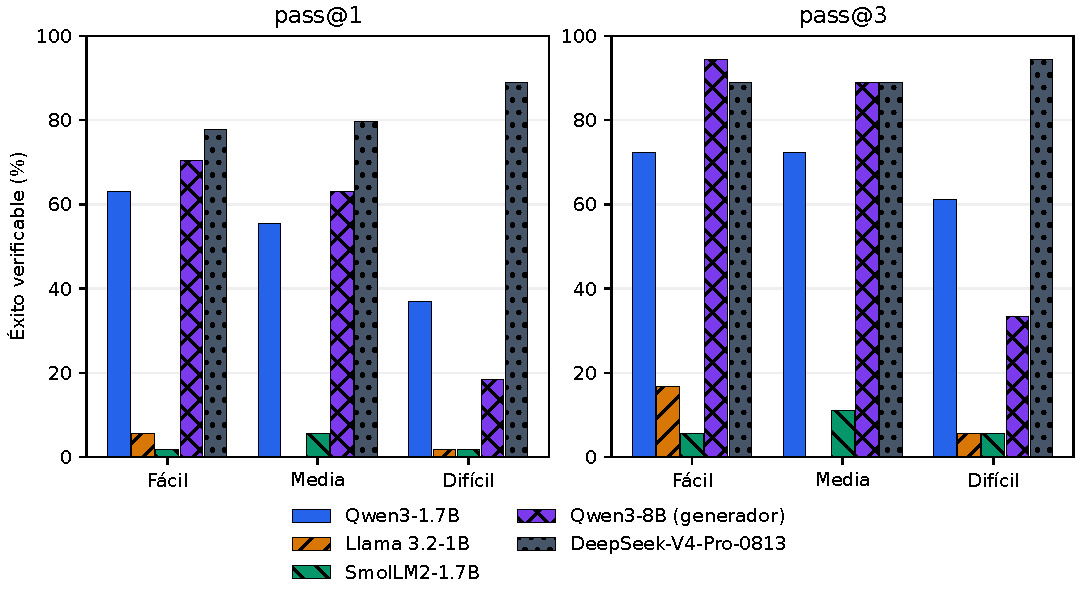
\includegraphics[width=\linewidth]{final-v2/figures/baseline.pdf}
\caption{Evaluación con verificador común por dificultad. Cada nivel contiene
18 tareas y 54 respuestas por modelo.}
\end{figure}

En el objetivo, pass@1 es 62,96\% en fácil, 55,56\% en media y 37,04\% en
difícil, y por familia alcanza 87,04\% en velocidad, 55,56\% en energía y
12,96\% en luminosidad. El promedio oculta, por tanto, una concentración de
fallos en esta última familia. Ni el objetivo ni Llama tuvieron truncamientos
o intentos incompletos, mientras SmolLM2 registró diez truncamientos y un
intento incompleto entre sus 162 respuestas. Su cobertura de 23,46\% y cota
optimista de 79,63\% hacen que el pass@1 automático de 3,09\% describa el
sistema bajo este formato, sin aislar capacidad matemática. Sus cinco aciertos
son de velocidad. Por su parte, Qwen3-8B obtuvo 82 aciertos, 74 errores
numéricos y seis no interpretadas, con pass@1 de 50,62\%, pass@3 de 72,22\%
y cobertura de 96,30\%, sin truncamientos ni intentos incompletos. La diferencia
frente a los 84 aciertos del objetivo no demuestra superioridad estadística
sobre esta muestra pequeña y relacionada.

Las 648 respuestas locales sumaron 2788,28 segundos de solicitudes y 153259
tokens de salida reportados. El intento incompleto de SmolLM2 no informó tokens
y se conserva como dato faltante. Por modelo, Qwen3-1.7B consumió 435,12 s y
31521 tokens, Llama 395,58 s y 26414, SmolLM2 869,42 s y 71009, y Qwen3-8B
1088,16 s y 24315. No hubo cargos de API local y no se midió electricidad.
Ollama informó que la memoria del modelo residió completamente en GPU en
las 162 observaciones de cada modelo, lo que no equivale a medir toda la
memoria del proceso ni el tamaño de los pesos en disco.

Las respuestas permiten distinguir errores de cálculo de límites del verificador.
En Qwen3-1.7B, una solución suma 2,936 y 0,734 km, convierte a 3670 m y
divide por 150 s para obtener 24,47 m/s correctamente. Otra trata 0,25 min
como 0,25 s y produce un resultado 60 veces mayor. En energía, 1022,27 J
se acepta frente a 1016,452 J por quedar dentro del 1\%, aunque la multiplicación
explicada sea incorrecta. En luminosidad, una respuesta termina en 30,7876 W
correctamente pero afirma que 1 W equivale a 1000 erg/s, mostrando que acertar
el valor final no certifica el razonamiento dimensional. También hay desarrollos
coherentes que quedan no interpretados por su formato LaTeX.

Estos ejemplos ilustran comportamientos, sin estimar su frecuencia ni corregir
manualmente las métricas. La baja cobertura de Llama, particularmente en
luminosidad, impide atribuir todos sus fallos a capacidad matemática. Además,
las diferencias de cuantización, formato de conversación, idioma y configuración
de pensamiento limitan la atribución causal de resultados al tamaño del modelo.
Para ampliar la comparación se evaluó también una referencia externa bajo las
mismas tareas y reglas de verificación.

\subsection{Referencia externa}
DeepSeek-V4-Pro-0813~\cite{deepseek} se ejecutó mediante OpenRouter con el
proveedor DeepInfra FP8 fijado, sin sustituciones automáticas y con presupuesto
de USD 5. Antes del test se realizaron cinco controles independientes que dieron
tres aciertos y dos respuestas no interpretadas, sin truncamientos, por
USD 0,0029965, y no se ajustó el extractor a esos resultados.

Se mantuvieron los 54 enunciados, tres muestras por tarea y la configuración
de muestreo local con semillas 42--44, máximo de 1024 tokens y razonamiento
desactivado, sin herramientas ni JSON forzado. El servicio anuncia contexto de
1048576 tokens frente a 2048 locales, y la identificación de los pesos se limita
al modelo fechado y proveedor, sin huella digital verificable. FP8 es la precisión
anunciada por el proveedor. Estas diferencias impiden asumir que iguales
parámetros produzcan un muestreo idéntico entre ejecuciones locales y remotas.

El test produjo 133 aciertos y 29 respuestas no interpretadas, con pass@1 de
82,10\%, pass@3 de 90,74\% y cobertura de 82,10\%. No se clasificaron errores
numéricos ni de unidad, ni hubo truncamientos o intentos incompletos, pero las
no interpretadas impiden concluir exactitud matemática perfecta y elevan ambas
cotas optimistas al 100\%. Fácil, media y difícil alcanzaron respectivamente
77,78\%, 79,63\% y 88,89\% en pass@1, confirmando que los niveles no ordenan
universalmente el rendimiento. Entre los falsos negativos hay una respuesta
correcta de 410,6 km/h que se rechaza porque mencionar que pi no se usa activa
una regla conservadora de negación, y otra con JSON correcto tras un marcador
narrativo sin cantidad. Ambas conservan su clasificación automática.

Las 162 solicitudes consumieron 25377 tokens de entrada y 22125 de salida,
sin tokens de razonamiento reportados, en 341,14 s. El test costó USD 0,0905151
y el total con controles fue USD 0,0935116. La tarifa capturada era
USD 1,30/2,60 por millón de tokens de entrada/salida~\cite{routing,pricing}.
El gasto efectivo quedó por debajo del presupuesto autorizado de USD 5.

\section{Reproducción}
El paquete incluye el informe, código y pruebas, tareas en \path{data/tasks/}
y soluciones SFT y pares DPO en \path{data/training/}. Las respuestas y
configuraciones de \path{results/} permiten recalcular la línea base y la
calibración, mientras las generaciones originales y auditorías permiten
reconstruir la selección SFT/DPO. Se conservan estos resultados como evidencia
necesaria para contrastar las cifras, sin incluir el historial de desarrollo.

README explica el contenido y el uso inicial, y REPRODUCING detalla cómo
comprobar integridad, regenerar tareas y reproducir datos derivados y métricas
desde una copia aislada. El código usa la biblioteca estándar de Python 3.12
y no requiere pesos ni credenciales para estas comprobaciones. Una nueva
inferencia sí necesita los modelos y motores identificados y puede dar respuestas
distintas aun con las mismas semillas, sin equivaler al recálculo aquí descrito.

\begingroup\raggedright
\begin{thebibliography}{9}
\bibitem{reasoninggym} Z. Stojanovski, O. Stanley, J. Sharratt, R. Jones,
A. Adefioye, J. Kaddour y A. K\"opf. Reasoning Gym: Reasoning Environments
for Reinforcement Learning with Verifiable Rewards. arXiv:2505.24760, 2025.
\url{https://arxiv.org/abs/2505.24760}.
\bibitem{gsmsymbolic} I. Mirzadeh, K. Alizadeh, H. Shahrokhi, O. Tuzel,
S. Bengio y M. Farajtabar. GSM-Symbolic: Understanding the Limitations
of Mathematical Reasoning in Large Language Models. arXiv:2410.05229, 2024.
\url{https://arxiv.org/abs/2410.05229}.
\bibitem{qwen17} Qwen. Qwen3-1.7B, model card oficial. Hugging Face,
\texttt{Qwen/Qwen3-1.7B}. Consulta: 7 de noviembre de 2026.
\bibitem{qwen8} Qwen. Qwen3-8B, model card oficial. Hugging Face,
\texttt{Qwen/Qwen3-8B}. Consulta: 7 de noviembre de 2026.
\bibitem{llama} Meta. Llama-3.2-1B-Instruct, model card oficial. Hugging Face,
\texttt{meta-llama/Llama-3.2-1B-Instruct}. Consulta: 7 de noviembre de 2026.
\bibitem{smol} Hugging Face. SmolLM2-1.7B-Instruct, model card oficial.
\texttt{HuggingFaceTB/SmolLM2-1.7B-Instruct}. Consulta: 7 de noviembre de 2026.
\bibitem{deepseek} DeepSeek / OpenRouter. DeepSeek V4 Pro 0813.
\url{https://openrouter.ai/deepseek/deepseek-v4-pro-20260813}.
Consulta: 7 de noviembre de 2026.
\bibitem{routing} OpenRouter. Provider Routing.
\url{https://openrouter.ai/docs/guides/routing/provider-selection}.
Consulta: 7 de noviembre de 2026.
\bibitem{pricing} OpenRouter. Pricing.
\url{https://openrouter.ai/pricing}. Consulta: 7 de noviembre de 2026.
\end{thebibliography}
\endgroup
